\subsection{Параллактический эллипс}
Движение Земли по орбите вокруг Солнца, очевидно, сопровождается изменением видимого положения объектов вне Солнечной системы. В приближении круговой орбиты, движение Земли циклично, а значит, траектории объектов относительно геоцентрической системы координат также цикличны. Чтобы установить, что из себя представляют данные траектории необходимо спроецировать годичное движение Земли на плоскость, перпендикулярную лучу зрения на объект.

Проекция окружности всегда эллипс, кроме вырожденного случая~--- отрезка, когда угол проекции составляет $90^\circ$. Так как проецирование с углом $\eta$ между плоскостями~--- тоже самое, что сжатие с коэффициентом $1/\cos\eta$.

Траектория Земли для наблюдателя, находящегося в окрестности объекта,~--- эллипс. Тогда понятно, что траектория объекта для наблюдателя на Земле также является эллипсом. Причем большая полуось этого эллипса равна параллаксу объекта $\pi = a_\oplus / r$, где $r$~--- гелиоцентрическое расстояние до объекта. А малая полуось равна
\begin{equation*}
	\pi' = \frac{a_\oplus \cos \eta}{r}.
\end{equation*}

\begin{figure}[h!]
	\centering
	\begin{tikzpicture}
		\footnotesize
		
		\coordinate (O) at (0, 0) {};
		\coordinate (A1) at (-0.57, 0.98) {};
		\coordinate (A2) at (0.57, -0.98) {};
		\coordinate (B1) at (-3, 0) {};
		\coordinate (B2) at (3, 0) {};
		\coordinate (C1) at (1.5, 2.6) {};
		\coordinate (C2) at (-1.5, -2.6) {};

		\draw (O) ellipse(3 and 1);
		\draw (O) [rotate=60] ellipse(3 and 1);
		\draw (O) [rotate=60] ellipse(1.5 and 1);
		
		\draw [dashes] (C1) -- (C2);
		\draw [dashes] (B1)  -- (B2);
		\draw (A1) -- (A2);
		
		
			\foreach \x in {-3, -2.9,...,3} {
				\draw [line width=.1pt] (\x, -3) -- (\x, 3);
			};
		
			\foreach \x in {-3, -2,...,3} {
				\draw [line width=.4pt] (\x , -3) -- (\x , 3);
			};
		
			\foreach \y in {-3, -2.9,...,3} {
				\draw [line width=.1pt] (-3, \y) -- (3, \y);
			};
			
			\foreach \y in {-3, -2,...,3} {
				\draw [line width=.4pt] (-3, \y) -- (3, \y);
			};
			
		\draw (A1) [fill=white] circle (.03);
		\draw (A2) [fill=white] circle (.03);
		\draw (B1) [fill=white] circle (.03);
		\draw (B2) [fill=white] circle (.03);
		\draw (O) [fill=white] circle (.03);
		
	\end{tikzpicture}
	\caption{}
\end{figure}

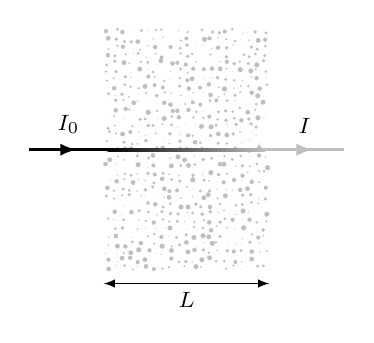
\begin{tikzpicture}
	\footnotesize

	\foreach \x in {-1, -.9, ..., 1.01} {
		\foreach \y in {-1.5, -1.4, ..., 1.51} {
			\pgfmathsetmacro\radius{(rand+1)/60};
			\fill [lightgray] (\x + rand*.03, \y + rand*.03)  circle(\radius);
		};
	};
	
	\draw [line width=1pt](-2, 0) -- (-1, 0);
	\draw [line width=1pt, -latex](-2, 0) -- (-1.4, 0);
	\draw [line width=1pt, lightgray](1, 0) -- (2, 0);
	\draw [line width=1pt, lightgray, -latex](1, 0) -- (1.6, 0);
	
	\fill[left color=black, right color=lightgray] (-1, -.5pt) rectangle (1, .5pt);
	
	\draw (-1.5, .1) node[anchor=south] {$I_0$};
	\draw (1.5, .1) node[anchor=south] {$I$};
	
	\draw [latex-latex] (-1.05, -1.7) -- (1.05, -1.7);
	\draw (0, -1.7) node[anchor=north] {$L$};
\end{tikzpicture}

Траектория (эллипс) видимого годичного движения объектов называется \term{параллактическим эллипсом}. Эксцентриситет параллактического эллипса можно найти из его его большой полуоси $\pi$ и малой~---~$\pi'$:
\begin{equation*}
	e 
	= \sqrt{1 - \left(\frac{\pi'}{\pi} \right)^2} 
	= \sqrt{1 - \left( \frac{r \cdot a_\oplus \cos \eta}{a_\oplus \cdot r}\right)^2} 
	= \sqrt{1 - \cos^2 \eta} = \sin \eta = \cos \beta,
\end{equation*}
где $\beta$~--- эклиптическая широта объекта.

